\documentclass[conference]{IEEEtran}
\IEEEoverridecommandlockouts
% The preceding line is only needed to identify funding in the first footnote. If that is unneeded, please comment it out.
\usepackage{cite}
\usepackage{amsmath,amssymb,amsfonts}
\usepackage{algorithmic}
\usepackage{graphicx}
\usepackage{textcomp}
\usepackage{xcolor}
\def\BibTeX{{\rm B\kern-.05em{\sc i\kern-.025em b}\kern-.08em
    T\kern-.1667em\lower.7ex\hbox{E}\kern-.125emX}}


\newcommand{\vectorsym}[1]{\ensuremath{\mathbf{#1}}}
\newcommand{\xextremum}{\ensuremath{x_{\mathrm{ext}}}}
\newcommand{\ccrit}{\ensuremath{c_{\mathrm{crit}}}}
\newcommand{\agentimpact}{\ensuremath{e}}
\newcommand{\empowerment}{\ensuremath{\mathfrak{E}}}
\newcommand{\sustainableempowerment}{\ensuremath{\empowerment^{\mathrm{sust}}}}
\newcommand{\setsymbol}[1]{\ensuremath{\mathcal{#1}}}
\newcommand{\stateset}{\ensuremath{\setsymbol{S}}}
\newcommand{\couplingconstant}{\ensuremath{d}}
\newcommand{\couplingfunction}{\ensuremath{C}}
\newcommand{\sumderivsquares}{\ensuremath{T}}
\newcommand{\impactstrength}{\ensuremath{E}}


\begin{document}

\title{Quantifying Sustainability in a System of Coupled Tipping Elements}

\author{\IEEEauthorblockN{1\textsuperscript{st} Jan T Kim}
\IEEEauthorblockA{\textit{School of Physics, Engineering and Computer Science} \\
\textit{University of Hertfordshire}\\
Hatfield AL10 9AB, UK \\
j.t.kim@herts.ac.uk}
\and
\IEEEauthorblockN{2\textsuperscript{nd} Daniel Polani}
\IEEEauthorblockA{\textit{School of Physics, Engineering and Computer Science} \\
\textit{University of Hertfordshire}\\
Hatfield AL10 9AB, UK \\
d.polani@herts.ac.uk}
}

\IEEEoverridecommandlockouts
\IEEEpubid{\makebox[\columnwidth]
{978-1-7281-2547-3/20/\$31.00 \copyright2020 Crown \hfill}
\hspace{\columnsep}\makebox[\columnwidth]{ }}
% Add the following code after the \maketitle command:
\IEEEpubidadjcol

\maketitle

\begin{abstract}
  Characterising sustainability has become a core challenge when
  trying to understand the interplay between global economical and
  ecological dynamics and both their mutual dependence as well as
  their competing requirements. Identifying and understanding warning
  signs that would indicate where when a system gets irrevocably out
  of control \emph{before} this happens would be a critical tool in
  being able to attain a viable long-term strategy that takes the
  needs of both economy and ecology into account.

  We here explore a route towards such  quantities. In the last years,
  the concept of \emph{empowerment} has been investigated as a measure
  of control of an actor over its environment, i.e.\ the potential
  impact that an actor can have on its environment; in addition an
  extension had been proposed towards a concept of \emph{sustainable
    empowerment} which, in addition, limits oneself only to control
  strategies which can be undone.

  We investigate both concepts inside a framework of systems of
  coupled elements endowed with a dynamics governed by cubic
  differential equations, which have been established as simple but powerful
  models to study sustainability. %   This enables characterising
  % sustainability as empowerment, a property emerging from the
  % interaction between the agent and the ecological systems sustaining
  % it.
  In this framework, we illustrate how the dynamical properties of
  such a system affect empowerment and sustainable empowerment. The
  results suggest that these quantities can provide relevant
  indicators for desirable strategies to guiding such systems under
  sustainability considerations.
\end{abstract}

\begin{IEEEkeywords}
sustainability, empowerment, information theory, dynamical systems
\end{IEEEkeywords}


\section{Introduction}

Sustainability is widely recognised as a central concept that should
underpin decisions and policies, aiming to ensure continued survival,
welfare and prosperity of humankind. In some contrast to its perceived
importance, a rigorous and generally applicable definition of
sustainability continues to prove elusive. Some approaches to define
sustainability, such as the Brundtland report that describes
sustainable development as ``development that meets the needs and
aspirations of the present without compromising the ability to meet
those in the future''\cite{Brundlandcommission1987}, are frequently
invoked in specific context (such as marine ecosystem protection).
However, they have not been formalised to enable unified application
to systems in general in ecology, economics, society and also
including Artificial Life models.

Ecosystem stability is a prerequisite for sustainability in the sense
that it is necessary to provide resources or ecosystem services (such
as air or water purification, climate regulation, or replenishment of
marine life used for food) on a permanent basis. An individual
resource can be considered to be used sustainably if it is regenerated
at a rate that (at least) matches the rate at which it is exploited.
This idea underpins methods for measuring footprints
\cite{Wackernagel2019_defyingthefootprintoracle}, which can be
aggregated over a key set of resources to calculate e.g.\ Earth
Overshoot
Day\footnote{https://www.footprintnetwork.org/2020/06/05/press-release-june-2020-earth-overshoot-day/}.

Stability is not a sufficient condition for sustainability, however.
States that are very stable can be unviable or undesirable, and
therefore may be considered unsustainable. As an example, the main
concern about global warming is the disruption it would cause to human
economy and society, not that a warmer global climate would be less
stable.

A considerable proportion of sustainability work focuses on
conservation of natural systems by reducing footprints of
exploitation, pollution and degradation, e.g.\ the Planetary
Boundaries
framework \cite{Steffen2015_planetaryboundaries}
% \footnote{https://www.stockholmresilience.org/research/planetary-boundaries/planetary-boundaries/about-the-research/the-nine-planetary-boundaries.html}
implicitly assumes that there are fixed boundaries of (regenerative)
capacity, and that resource consumption or depletion needs to be
reduced where these boundaries are exceeded. However, for some
resources, boundaries of production or regeneration rates can be
greatly expanded. The most dramatic example of this is arguably
production of staple foods, which has increased by orders of magnitude
since agriculture was first adopted, enabled by technologies including
fertilisers and plant breeding, and culminating in the Green
Revolution. The resulting agricultural systems are stable only by
continued management. If human impact were removed, they would change
to a more stable state by ecological succession e.g.\ from farmland to
forest.

These observations highlight that the entity being sustained is
central to the concept of sustainability, even though this entity,
typically humankind or a group of stakeholders, is frequently
implicitly assumed rather than stated expressly. A stable state of the
planet that is inhospitable to human life, or disruptive to
socio-economic systems, is generally considered unsustainable. On the
other hand, forcing a system into an altered state is in many cases
considered sustainable, so long as such impacts can be controlled and
they are associated with beneficial and desirable effects. As an
example, sustainable agricultural production processes can be
characterised as cycles of forcing changes to ecosystems from this
perspective.

Empowerment provides a method to quantify the control of an agent over
its environment, i.e.\ its ability to influence or force the
environment's state. Formally, for an agent interacting with an
environment via a sensor and an actuator, empowerment is defined as
the amount of Shannon information transmitted from the actuator via
the environment to the sensor \cite{Klyubin2005_beempowered}. In a
fully deterministic system, empowerment turns out to be the Shannon
entropy of the uniform distribution across all states that are
reachable and distinguishable by the agent. It is important to note
that the uniform distribution applies to the reachable states,
\emph{not} the action sequences taken by the agent.

% todo: fruit successions?

% todo: family silver

% introduce tipping systems

% discuss problems of "unwanted" / "unsustainable" stable fixed points

% More formal approaches to sustainability often focus on stability.
% While stability of the sustaining environment (e.g.\ the planet with
% its ecological and abiotic systems) is necessary for
% sustainability, focusing on it alone excludes the active role of the
% entity seeking to be sustained (e.g.\ humankind).

In previous work, we have modified empowerment to quantify
sustainability by constraining the states to those for which the agent
is able to bring the system back to the start state
\cite{Kim2009_sustainability}. In this case, the agent is able to
operate a cycle which is a simple model of a sustainable process e.g.\
as outlined for agriculture above. On the other hand, bringing the
system into a state for which there is no way back corresponds to
unsustainable practices such as using non-renewable resources.

Stability and control over a system can collapse dramatically at
critical points in system dynamics
\cite{Lenton2019_riskytippingpoints}. Such tipping elements have been
modelled by bi-stable systems in which perturbations of sufficient
strength can result in transition from one state to another
\cite{Lenton2008_tippingelements}. Cubic differential equations
capture this key property, and they have been used as building blocks
for models in which multiple tipping systems are coupled
\cite{Brummitt2015_coupledcatastrophes,Klose2019_interactingtippingelements}.

Multistability and a potential of tipping occur in a wide range of
real world systems, and for most of these, cubic differential
equations are at most a qualitative model. Nonetheless, coupled cubic
equations are a powerful and convenient modelling tool that is able to
capture cascades of tipping and other complex phenomena. Here, we use
them as a framework to explore and demonstrate properties of
empowerment-based sustainability in a model environment that
qualitatively reflects some of the tipping point dynamics of the
systems sustaining humankind on Earth.

% explain that cubic equation systems have been used to explore
% sustainability, but so far the agent to be sustained has not been
% expressly included in such approaches.

% related to May1972: how to determine matrix A? Related to, but not
% identical to interaction matrix in cubic system --> distribution of
% values and calculation of May's \alpha may not be entirely
% straightforward. Note that A depends on current state (local) while
% cubic interaction terms are global.

% Ideas: Demo variant of Brummitt et.al.'s hopping and discuss
% sweep interaction strength and empowerment, look for relation to
% May1972 etc.
% todo: final paragraph leading in to the system


\section{System}

Our system consists of $n$ coupled elements, each of which has a state
$x_i \in \mathbb{R}$ which may be thought of as the abundance of e.g.\
a species or a resource. The state of the entire system is thus a
vector $\vectorsym{x} = (x_1, \ldots, x_n)^T \in \mathbb{R}^n$. The
temporal evolution of the system is determined by the intrinsic
dynamics of the environment and the impact of an agent. Formally, the
dynamics of each tipping element $i$ are determined by the differential
equation
\begin{equation}
  \label{eq_coupledwithagent}
  \frac{dx_i}{dt} = f(\vectorsym{x}) = x_i - x_i^3 + c_i + \couplingfunction_i(\vectorsym{x}) + \agentimpact_i(t)
\end{equation}
where $c_i$ is a random value that is drawn from a uniform
distribution centred on $0$ and constant for a given system,
$C(\vectorsym{x})$ characterises the coupling  between the elements, and $\agentimpact_i(t)$ is
 the agent impact which may be interpreted as the rate at
which a resource (e.g.\ biomass) is exploited or a substance (e.g.\
plastic, phosphates or other chemicals) is released into the
environment. The coupling function is given by
\begin{equation}
  \label{eq_couplingfunction}
  \couplingfunction_i(\vectorsym{x}) = \sum_j \couplingconstant_{ji} x_j
\end{equation}
where the coupling parameters $\couplingconstant_{ji}$ are drawn from a uniform
$0$-centred distribution for $j < i$ and set to $0$ otherwise, i.e.\
$(\couplingconstant_{ji})$ is an upper triangular matrix.

This design of the environment comprised of tipping elements governed
by cubic differential equations falls into the general class of models
reviewed by Klose \textit{et al.}\
\cite{Klose2019_interactingtippingelements}.

Restricting the interaction matrix $\couplingconstant_{ji}$ to an upper triangular
matrix means that an element $j$ will only act on elements $i$ with a
larger index, $i>j$, but
never will an element $i$ act on an element $j$ of lower index. In
particular,  the interactions between the elements form a
directed acyclic graph (DAG). % In other words, the interactions form a
% hierarchy in the sense that each element affects only those with an
% index greater than its own.
We chose this design because cyclic interactions qualitatively change
the ``tipping point'' characteristics of the elements, as discussed in
more detail below.

% todo: make sure loss of tipping point characteristics (cyclic
% attractors rather than fixed points etc) is discussed below.

% \begin{equation}
%   \label{eq_cubic}
%   \frac{dx}{dt} = ax - bx^3 + c
% \end{equation}
% As \cite{Klose2019_interactingtippingelements}, we restrict
% ourselves to $a = 1$ and $b = 1$.

% The state of a system of $n$ interacting tipping elements is a vector
% $\vectorsym{x} = [x_1, \ldots, x_n]^T$ whose interaction is modelled
% by a diff

%  a coupling function $\couplingfunction_i(\vectorsym{x})$
% \begin{equation}
%   \label{eq_coupled}
%   \frac{dx_i}{dt} = ax_i - bx_i^3 + c_i + \couplingfunction_i(\vectorsym{x})\;.
% \end{equation}
% Following \cite{Klose2019_interactingtippingelements}, we use coupling
% functions
% \begin{equation}
%   \label{eq_couplingfunction}
%   \couplingfunction_i(\vectorsym{x}) = \sum_j \couplingconstant_{ji} x_j
% \end{equation}
% but unlike their work, we require $\couplingconstant_{ji} = 0$ if $j \ge i$,
% i.e.\ $(\couplingconstant_{ij})$ to be a lower triangular matrix. This restriction
% ensures that, for coupled tipping elements, their bi-stable character
% is preserved (bi-directional interactions between tipping elements can
% result in global dynamical features that amount to a qualitative
% departure from the ``tipping point'' system characteristics, such as
% cyclic attractors). Thus the graph of interactions becomes a directed
% acyclic graph, in which we can arrange the components in order, so
% that the steady state of component $x_i$ depends only on higher-ranked
% components $x_1, \ldots x_{i-1}$, enabling efficient computation of
% fixed points of the system. This models an interrelated, but
% hierarchical ``ecosystem'' with different levels of importance for the
% subsystems.  Model now the additional effect of the agent
% (``humanity'') on its environment by the totality of the terms
% $\agentimpact_i(t)$:
% \begin{equation}
%   \label{eq_coupledwithagent}
%   \frac{dx_i}{dt} = ax_i - bx_i^3 + c_i + \couplingfunction_i(\vectorsym{x}) + \agentimpact_i(t)
% \end{equation}
% This affects the rate of change in the $x_i$; examples would be modelling
% emissions of carbon dioxide, release of nutrients
% (e.g.\ phosphates), or removal of biomass (harvesting).


\subsection{System Properties}

\begin{figure}

  \centerline{\includegraphics[width=6cm]{cubicdemo_intercept000.eps}}

  \centerline{\includegraphics[width=6cm]{cubicdemo_intercept025.eps}}

  \centerline{\includegraphics[width=6cm]{cubicdemo_intercept100.eps}}

  \caption{Illustrations of stable fixed points in cubic differential
    equations. Fixed points $x_{-}$ and $x_{+}$ are shown as blue. The
    blue lines indicate the gradients at the fixed points. Extrema are
    shown in red. The intercept
    $\Delta dx_i / dt := c_i + \couplingfunction_i(\vectorsym{x}) + \agentimpact_i(t)$ is
    shown as a dark grey bar. Top: At $\Delta dx_i / dt = 0$,
    gradients at both fixed points are equal. Middle: At
    $0 < \Delta dx_i / dt < \ccrit$, the gradient at $x_{-}$ is flatter
    while that at $x_{+}$ is steeper. Bottom: At
    $\Delta dx_i / dt > \ccrit$, $x_{-}$ disappears while the steepness
    at $x_{+}$ increases.}
  \label{fig_cubicdemo}

\end{figure}

Each element in our system has one or two stable fixed points. For the
special case of
$c_i = 0, \couplingfunction_i(\vectorsym{x}) = 0, \agentimpact_i(t) = 0$, there are two
stable fixed points which can be straightforwardly found as
$x_{-} = -1$ and $x_{+} = 1$. The local extrema in this special case
can be found at $\pm \xextremum = \pm 1 / \sqrt{3}$, and the rate of
change at these extrema evaluates to
$\pm d\xextremum / dt = \pm \ccrit = \pm 2 / 3\sqrt{3} \approx \pm
0.38$.

In the general case, $c_i$, $C(\vectorsym{x})$ and $\agentimpact_i(t)$
take on arbitrary values, shifting the cubic function along the
$dx / dt$ (vertical) axis while the extrema remain unchanged, and consequently,
the stable fixed points are constrained to $x_{-} < -\xextremum$ and
$x_{+} > \xextremum$ respectively. Element $i$ has two stable fixed
points if
$-\ccrit < c_i + \couplingfunction_i(\vectorsym{x}) + \agentimpact_i <
\ccrit$,
as illustrated in Fig.~\ref{fig_cubicdemo}. Elements also have an
unstable fixed point, which merges into a semi-stable fixed point in
the corner cases of
$c_i + \couplingfunction_i(\vectorsym{x}) + \agentimpact_i = \pm
\ccrit$.
It is worth noting that the unstable fixed point is the boundary
between the basins of attraction of the stable fixed point. Klose et
al.\ \cite{Klose2019_interactingtippingelements} refer to $x_{-}$ and
$x_{+}$ as the ``normal'' and the ``tipped'' state, respectively.

Fig.~\ref{fig_cubicdemo} also shows that as the intercept
$c_i + \couplingfunction_i(\vectorsym{x}) + \agentimpact_i(t)$
increases, the gradient of the cubic function gets flatter at $x_{-}$
and steeper at $x_{+}$. This gradient quantifies the speed with which
the tipping element returns to the fixed point after a small
perturbation, and it can therefore serve as an indicator of stability.
We therefore characterise stability of a fixed point
$\vectorsym{x}_* = (x_{1*}, \ldots, x_{n*})^T$ with the sum of
derivative squares,
\begin{equation}
  \label{eq_dss}
  \sumderivsquares = \sum_i (1 - 3 x_{i*}^2)^2.
\end{equation}

Due to the DAG structure of interactions, the stable fixed points of
element $i$ only depend on the state of elements $1, \ldots, i - 1$.
This enables efficient computation of the stable fixed points of the
entire system.

If the intercept is constant, $\couplingfunction_i(\vectorsym{x})$
will converge as elements $1, \ldots, i - 1$ converge towards their
respective fixed points, which will facilitate convergence of element
$i$ as well. Allowing cyclic interactions would result in the
emergence of qualitatively different dynamics, such as cyclic
attractors. As a simple example, a two-element system with
$\couplingconstant_{12} = -\couplingconstant_{21}$ has a cyclic
attractor in which elements $1$ and $2$ oscillate between negative and
positive values.

From this perspective, restricting $(\couplingconstant_{ji})$ to an upper triangular
matrix of (randomly chosen) values can be considered to define a very
general class of coupled cubic differential equations in which all
elements retain the property of having two guaranteed stable fixed
points that can meaningfully be designated $x_{-}$ and $x_{+}$.


\subsection{Empowerment}
\label{section_empowerment}

\begin{figure}

  \centerline{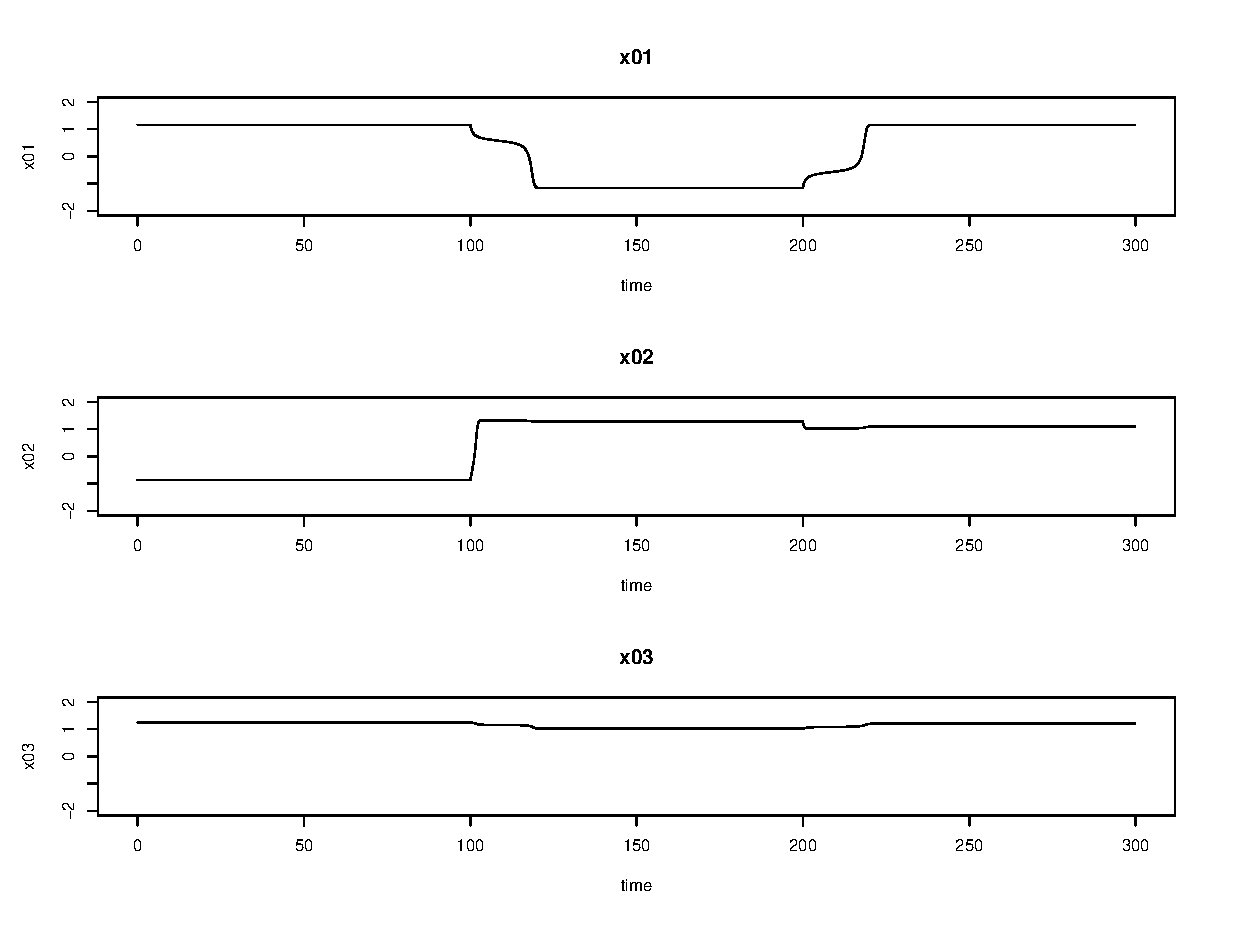
\includegraphics[width=8cm]{agentimpact_ode.eps}}

  \caption{Illustration of an agent impacting on an environment with
    three tipping elements. Initially, up to $t = 100$, the
    environment is at the stable fixed point
    $(x_{1+}, x_{2-}, x_{3+})$. The agent's impact is applied at
    $100 \le t < 200$, causing elements $1$ and $2$ to change their
    discretised state. After removing the agent's impact at $t = 200$,
    element $1$ returns to its initial state while element $2$ remains
    at $x_{2+}$. The gradual impact experienced by element $3$ do not
    amount to a change in discretised state. Simulation of the
    actuation shown here establishes that state
    $(x_{1+}, x_{2+}, x_{3+})$ is accessible from state
    $(x_{1+}, x_{2-}, x_{3+})$.}
  \label{fig_agentimpact}
\end{figure}

% \section{Combined Framework}

% We present now the core framework.
% An individual ``cubic tipping element'' as defined by
% Eq.~\eqref{eq_cubic} has one or two stable fixed points. In the simple
% special case of $c = 0$, there are two stable fixed points which can
% be straightforwardly found as $x_{-} = -1$ and $x_{+} = 1$,
% \cite{Klose2019_interactingtippingelements} refer to these as the
% ``normal'' and the ``tipped'' state, respectively. The third, unstable
% fixed point at $x_{\mathrm{unstable}} = 0$ is not important for the
% work presented here.

% The condition for an individual tipping element to have two stable
% fixed points can thus be stated more precisely as
% $-\ccrit < c < \ccrit$. This condition generalises to
% $-\ccrit < c + \couplingfunction_i(\vectorsym{x}) + \agentimpact_i < \ccrit$ for a
% tipping element $i$ in a system of coupled elements subject to impacts
% by the agent.

To compute empowerment in the tipping scenario, we determine the
potential stable points that can be ``intentionally'' induced by the
agent. We discretise the state of the environment by distinguishing
only the two stable states $x_{i+}$ and $x_{i-}$ for each element $i$,
resulting in a state set $\stateset$ with $|\stateset| \le 2^n$. We
consider a micromanaging agent which controls every
single impact $\agentimpact_i$ that each of the elements $i$ imposes on
the system. As in our previous work \cite{Kim2009_sustainability}, we
assume no noise in the agent sensing and actuation. Under these
assumptions, empowerment reduces to  the logarithm of the number of states
which the agent can reach by applying its
impact actuators $\agentimpact_i$.

We use the stable fixed points of the unimpacted environment, i.e.\
with $\agentimpact_i(t) = 0\; \forall i, t$, as starting points for
which we characterise empowerment. We allow the agent to impact the
environment by choosing to set $\agentimpact_i$ to $-\impactstrength$,
$0$ or $\impactstrength$, where $\impactstrength$ is a parameter
setting the strength of the impact, or control, of the agent on the
environment. A setting of
$\vectorsym{\agentimpact} = (\agentimpact_i, \ldots,
\agentimpact_n)^T$ is called an actuation.

If these controls were applied permanently and sufficiently large,
e.g.\ if one had
$\impactstrength \gg \ccrit + \max_i \couplingfunction_i$, the agent
could directly ``dial'' the state of each component, and consequently
its empowerment would attain the maximal value of $n$ bits. At the
other extreme, setting $\impactstrength = 0$ prevents the agent from
having any impact on the environment at all and would cause its
empowerment to vanish in all states.

A crucial issue concerning sustainability in general, and tipping
points in particular, is that human impact could result in changes to
the environment that are permanent, i.e.\ where discontinuing an
impact may not be sufficient to restore the environment to its
``normal'' state. Therefore, we only count state changes that persist
once the direct control of the agent is removed. We implement this by
letting the agent apply its impact for a limited time only, which is
followed by a relaxation period during which the environment evolves
on its own and converges towards one of its fixed points.
Fig.~\ref{fig_agentimpact} illustrates this process for a small
system.

A state $s'$ reached at the end of this relaxation period is defined
to be $\impactstrength$-accessible from the initial state $s$. We
consider this to be the state resulting from the agent's actions, and,
analogously to \cite[eq.~(2)]{Kim2009_sustainability}, we formally define
empowerment as
\begin{equation}
  \label{eq_empowerment}
  \empowerment(\impactstrength, s) =
  \log_2(|\{s': s' \mbox{ is } \impactstrength\mbox{-accessible from } s\}|)
\end{equation}
This corresponds to a maximum entropy distribution on the target
states (not on the actions), since there is no noise in our system.

In previous work, e.g.\ \cite{Salge2014_empowermentintro} the agent's
reach is typically restricted by imposing a time window for its
actions. Instead, here we use $\impactstrength$ to limit the range of
effects that the agent can cause. In our system, changes to the
equilibrium state in a tipping element are monotonic both with respect
to the direct impact via $\agentimpact_i$ and the indirect impact via
the coupling function $\couplingfunction_i(\vectorsym{x})$.
Consequently, the maximum of $|\agentimpact_i|$ during a time window
largely determines whether the agent's actions result in a change of
the discretised state of element $i$ while the details of the
trajectory by which the maximum is reached are irrelevant. Therefore,
limiting $\impactstrength$ directly is equivalent to imposing a time
window and boundaries on the rate with which the agent can change the
$\agentimpact_i$ values. As a technical advantage, limiting
$\impactstrength$ eliminates numerical integration over a time window
and thereby facilitates efficient computational exploration of the
system dynamics. Theoretically, it may be of interest that
appropriately limiting action range can serve as an alternative to
limiting time when applying empowerment.


% effect on the discretised state largely depends on the maximum of
% $\agentimpact_i$ during a given time period.

% Our
% rationale is

% A straightforward implementation of
% this approach would be to allow the agent to change its impacts on the
% tipping elements with a bounded rate
% $|d\agentimpact_i / dt| \le r_{\mathrm{max}}$ during a time window
% $[0, \timehorizon]$. This can be simplified by noticing that the
% change to the equilibrium state $x_i$ of tipping element $i$ is
% monotonic, both with respect to the direct impact $\agentimpact_i$ and
% the indirect impact via the coupling function
% $\couplingfunction_i(\vectorsym{x})$. As a consequence, the maximum
% change the agent can make to its actuation, i.e.\
% $r_{\mathrm{max}} \timehorizon$, determines its ability to tip an
% element.
% the detailed dynamics of the trajectories of $\agentimpact_i$ during
% the horizon time interval are inconsequential.

% Therefore, our definition of empowerment as a function of
% $\impactstrength$, which limits $|\agentimpact_i|$, i.e.\ the strength
% of the effect that the agent can exert on each of the tipping elements
% $i \in \{1, \ldots, n\}$, is analogous to assuming bounds on rates of
% impact and a limited time horizon. This approach has the technical
% advantage of enabling more efficient computational exploration, as
% detailed further in section \ref{section_implementation}. It is
% interesting to notice from a theoretical perspective, however, that
% defining an action horizon, as $\impactstrength$, rather than a
% narrower concept of a time horizon, is sufficient to apply
% empowerment.

% It is important to notice that an increasing
% range of $\agentimpact_i$, analogously to an increasing time horizon,
% results in increasing empowerment.

Empowerment as measured by \eqref{eq_empowerment} increases as the
number of accessible states grows. However, in some states, the agent
may be unable to meet some of its needs. If the agent brings the
environment into such a state permanently and irretrievably, that
would compromise the agent's ability to meet its needs in the future.
This would make an actuation (i.e.\ a way of using or interacting with
the environment) unsustainable in the sense of the Brundtland
report. However, if the agent is capable of returning the
environment into its initial state, the ability to meet its future
needs would not be compromised. This provides us with a criterion to
distinguish between sustainable and (potentially) unsustainable
actuations which does not require any external (and possibly arbitrary
or contentious) designation of states as sustainable or unsustainable.
Therefore, consistently with our previous work
\cite{Kim2009_sustainability}, we define a state $s'$ to be reversibly
accessible from a state $s$ if $s'$ is accessible from $s$ and $s$ is
accessible from $s'$. This allows us to apply our previous definition
of sustainable empowerment as
\begin{equation}
  \label{eq_sustainableempowerment}
  \begin{aligned}
    & \sustainableempowerment(E, s) = \\
    & \log_2(|\{s': s' \mbox{ is
      reversibly } E\mbox{-accessible from } s\}|).
  \end{aligned}
\end{equation}


\subsection{Implementation}

The software for the analyses presented here was written in R 3.4.4
\cite{RManual2018} and requires the \texttt{deSolve} package for
solving \eqref{eq_coupledwithagent} using Runge-Kutta 4th order
integration.

Computing empowerment and sustainable empowerment \eqref{eq_empowerment}
and sustainable empowerment \eqref{eq_sustainableempowerment} requires a
matrix of accessibility for all pairs of states $(s, s')$. The key
process in computing accessibility is to determine the fixed point
$s_{\vectorsym{\agentimpact}}$ reached with the agent impact active
when starting from state $s$, and to determine the final state $s'$
reached from $s_{\vectorsym{e}}$ after removing the agent impact.
Using numerical integration to compute accessibility is
computationally demanding, as it involves iterating over the Cartesian
product of all states and all actuations.

The DAG structure of interactions, in combination with limiting
$\impactstrength$ rather than using a time window, enables us to
approximately determine the state $s'$ reached after applying and
subsequently removing the agent's impact without numerical
integration. The coupling function
$\couplingfunction_i(\vectorsym{x}_*)$ depends only on
$x_{1*} \ldots, x_{i-1*}$. On this basis we can determine whether
$x_i$ is in the basin of attraction of $x_{-}$ or $x_{+}$, assuming
that the upstream elements $1, \ldots, i - 1$ have converged to the
fixed point already. This assumption is an approximation, as the
elements are following their respective trajectories simultaneously,
rather than converging sequentially.

Our approximation is most likely to result in errors when $x_i$ are
close to the boundary between basins of attraction. We expect that
this is a rare condition as the points visited during accessibility
matrix computation are not biased towards the basin boundaries. With
small $\impactstrength$, the fixed points with and without agent impact are similar,
so the starting points are in fact biased to be close to fixed points
and thus distant from boundaries. As $\impactstrength$ increases, starting points
cover a broader range and the bias towards fixed points diminishes.
The chance of generating starting points in the vicinity of attractor
basin boundaries can be expected to increase as a result, but
considering the overall dilution of probability density as ranges
broaden, that chance can be expected to remain small.

The code used to generate the results presented in this contribution
is available at \texttt{https://github.com/jttkim/al20sustain}.


\section{Results}

\begin{figure}
  \begin{center}

    \includegraphics[width=8cm]{n08_full_small_emp.eps}

    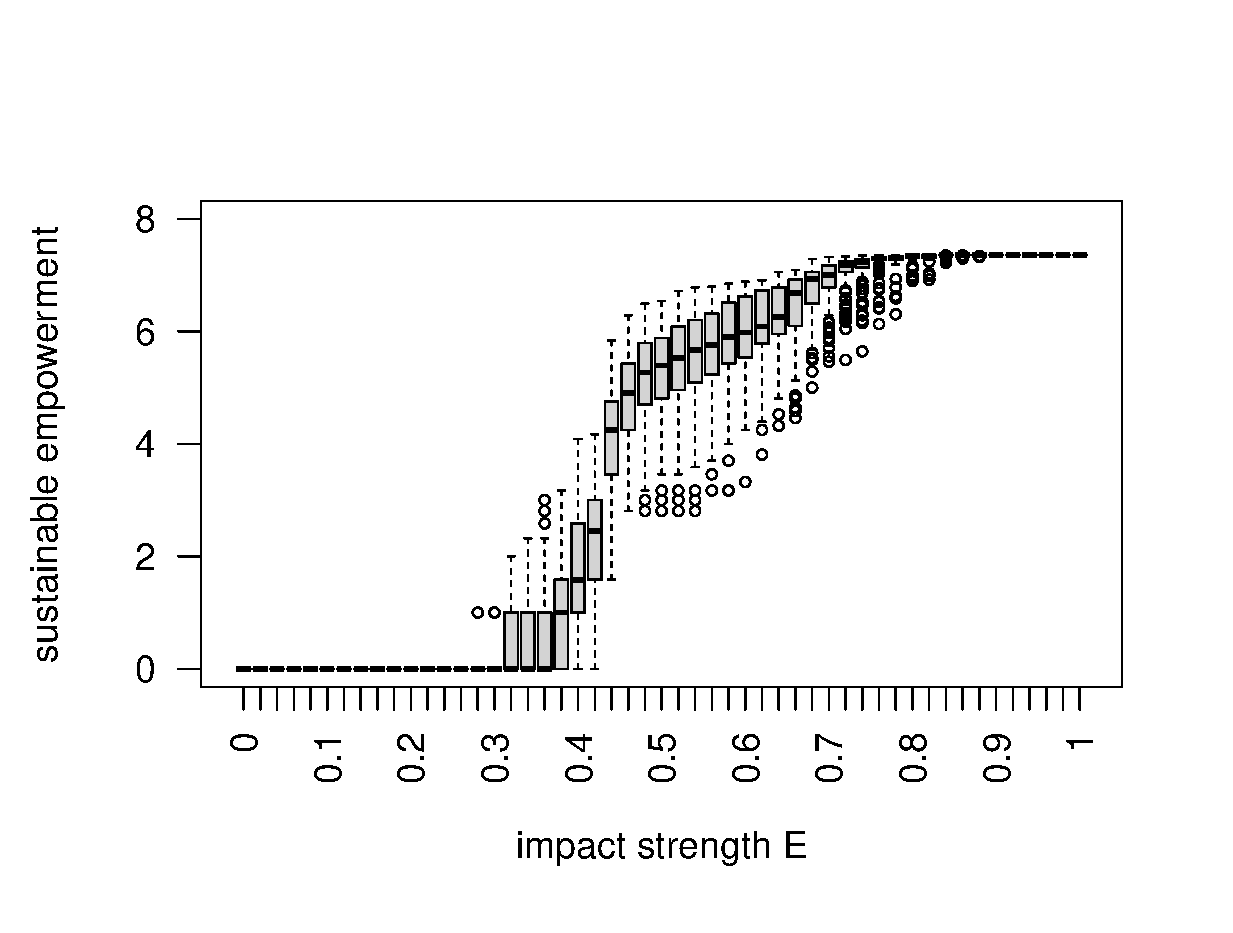
\includegraphics[width=8cm]{n08_full_small_empsust.eps}

  \end{center}

  \caption{Empowerment (top panel) and sustainable empowerment
    (bottom panel) as a function of $\impactstrength$. Each boxplot summarises
    sustainability values for all initial states. The middle bar of
    a box shows the median, the box indicates the central quartiles,
    whiskers extend to the furthest point less than 1.5 times the
    interquartile range, and points outside this range are plotted
    individually.}
  \label{fig_empowermentprofiles}
\end{figure}

We show results for a system of $8$ tipping elements, with values
$-0.1 \le c_i \le 0.1$ and $-0.2 \le \couplingconstant_i \le 0.2$
drawn from uniform random distributions.

Empowerment and sustainable empowerment as a function of impact
strength $\impactstrength$ are shown in
Fig.~\ref{fig_empowermentprofiles}. As explained in section
\ref{section_empowerment}, with $\impactstrength = 0$, empowerment is
$0$ for all states. As $\impactstrength$ increases, actuations can
facilitate access to other state and states with
$\empowerment(E, s) > 0$ appear. Further growth of $\impactstrength$
results in increasing empowerment of states as well as in the number
of states with a non-zero empowerment. As $\impactstrength$ approaches
$1$, all states become maximally empowered. The maximum remains below
$8$ because elements can have only one fixed point, and therefore not
all combinations in $\{-, +\}^{8}$ correspond to existing fixed
points.

The qualitative features of sustainable empowerment
$\sustainableempowerment$ as a function of $\impactstrength$ are
similar to those seen for $\empowerment$. The main differences are
that higher values of $\impactstrength$ are required to obtain
non-zero sustainable empowerment, and that higher values are also
required for states with submaximal empowerment to disappear. Both
these features are straightforwardly explained by the condition of
reversible accessibility which underpins sustainable empowerment and
is a stricter condition than plain accessibility.


\begin{figure}

  \begin{center}

    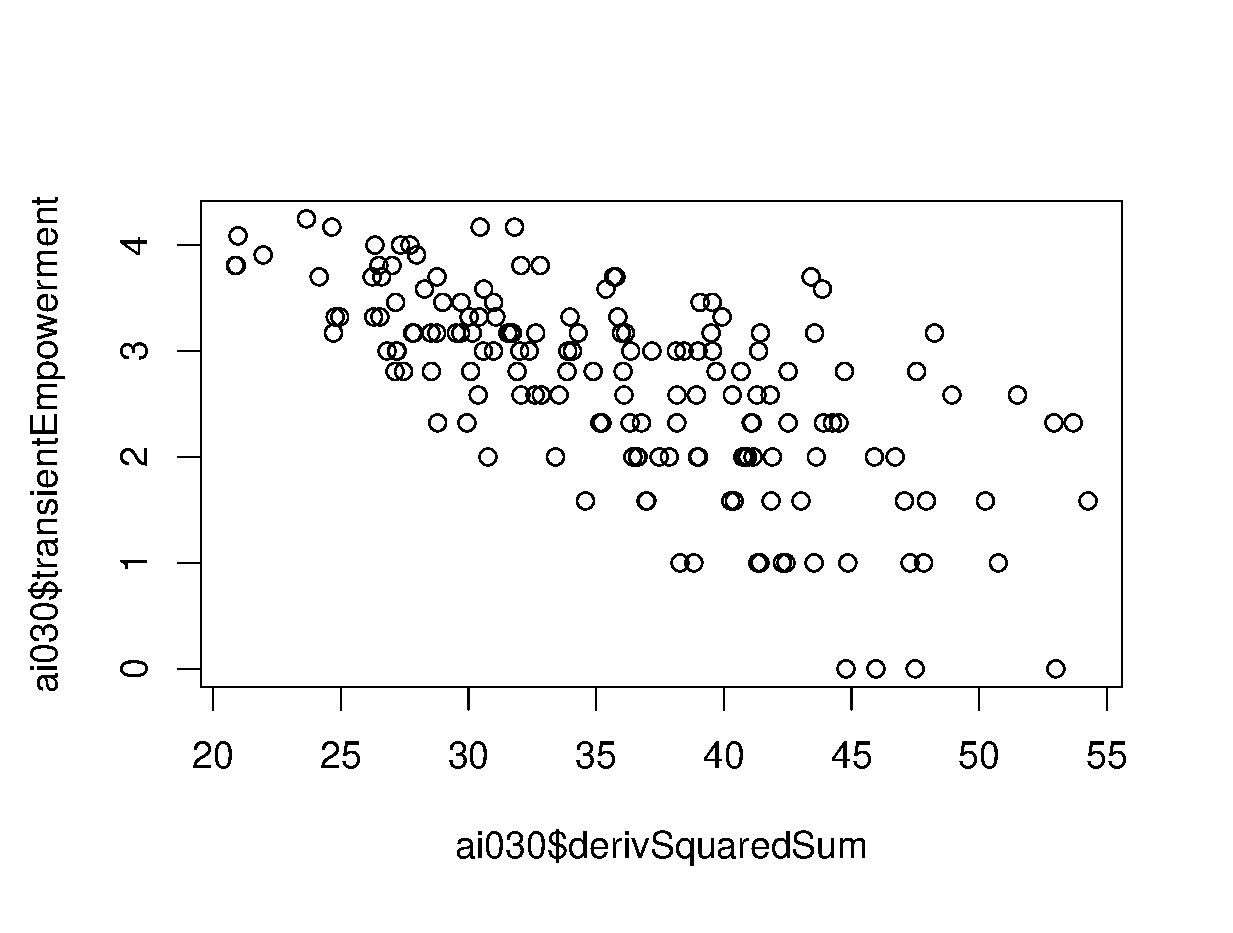
\includegraphics[width=8cm]{n08_full_small_corr_dss_emp_ai030.eps}

    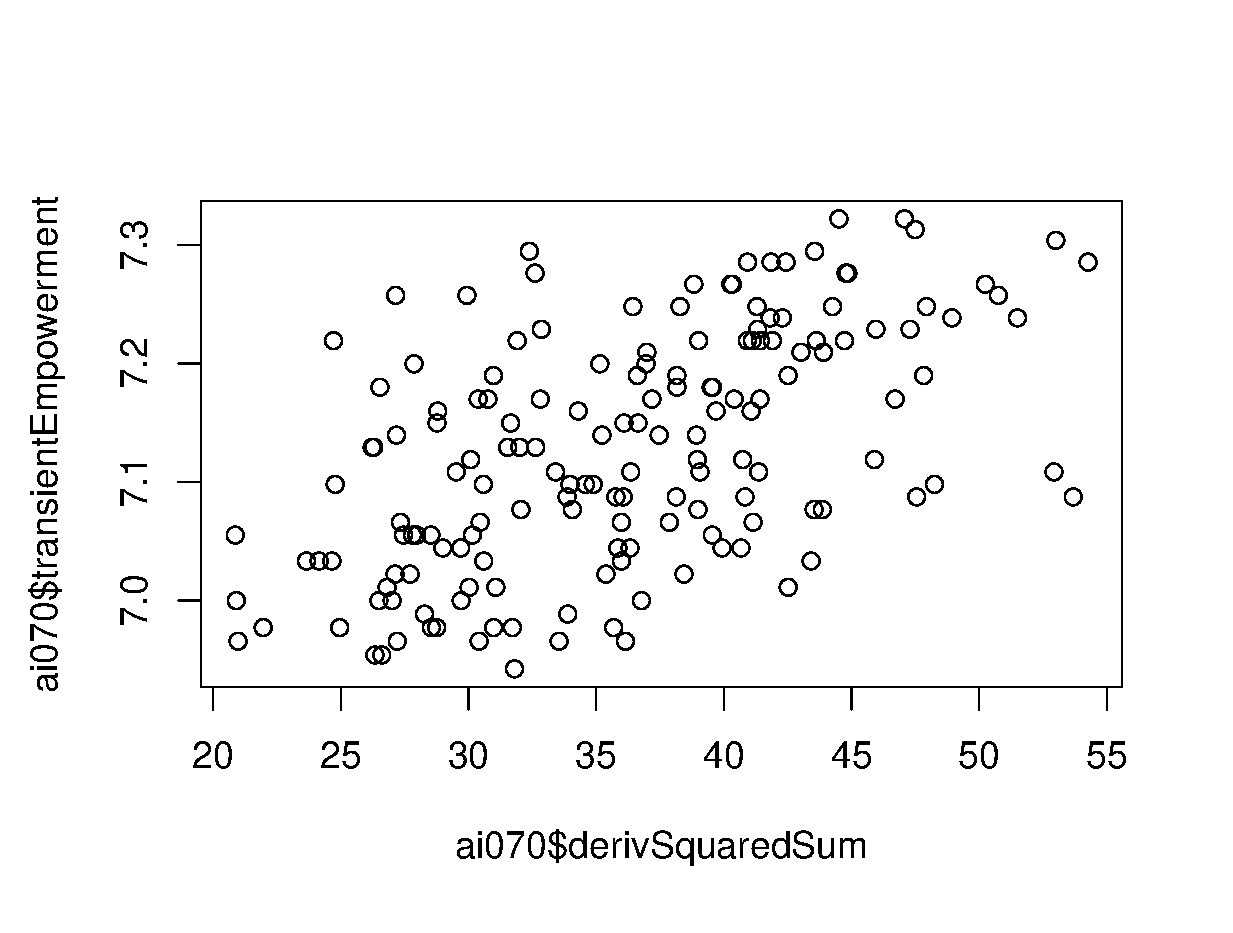
\includegraphics[width=8cm]{n08_full_small_corr_dss_emp_ai070.eps}

  \end{center}

  \caption{Scatterplot of the sum of derivative squares and
    empowerment at $\impactstrength = 0.3$ (top) and $\impactstrength = 0.7$ (bottom).}
  \label{fig_dssemp}

\end{figure}

We now turn to investigating relationships between empowerment and
stability. Fig.~\ref{fig_dssemp} shows scatterplots of the sum of
derivative squares $\sumderivsquares$, as defined in \eqref{eq_dss}.
At the smaller actuator range $\impactstrength = 0.3$, empowerment decreases as the
sum of derivative square increases. At the larger value $\impactstrength = 0.7$,
this trend reverses to a positive correlation.

\begin{figure}

  \begin{center}

    \includegraphics[width=8cm]{n08_full_small_corr_dss_emp.eps}

    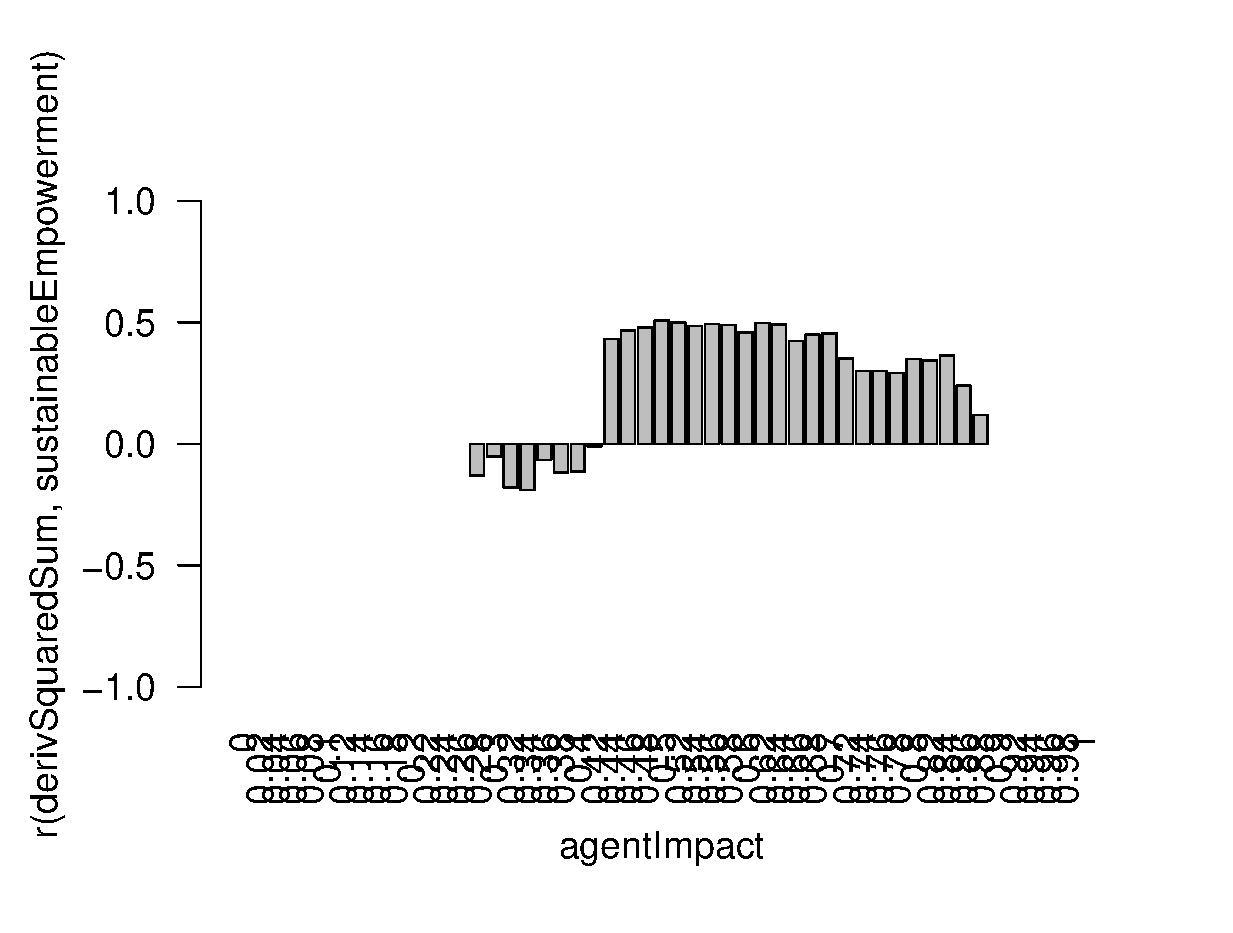
\includegraphics[width=8cm]{n08_full_small_corr_dss_empsust.eps}

  \end{center}

  \caption{Barplots of Pearson correlation coefficients between the
    sum of derivative squares and empowerment (top) and between the
    sum of derivative squares and sustainable empowerment (bottom). No
    bars are shown where correlation is undefined because the variance
    of empowerment is $0$.}
  \label{fig_dssempcorr}

\end{figure}

These two examples are illustrative of a general trend associated with
increasing impact strengths, as shown in Fig.~\ref{fig_dssempcorr}
which displays the Pearson correlation coefficients between
$\sumderivsquares$ and $\empowerment$ and $\sustainableempowerment$,
respectively.

A negative correlation between $\sumderivsquares$ and $\empowerment$
means that on average, more states are accessible from fixed points
with shallower gradients. At a small impact strengths, many actuations
do not result in a permanent change of state in a tipping element. As
illustrated in Fig.~\ref{fig_cubicdemo}, for a fixed point with a
shallower gradient, a smaller change in the intercept causes the fixed
point to vanish and thus the element to tip. Therefore, permanently
changing the state of elements with a shallower gradient is easier for
an agent with a weaker impact. This results in the negative
correlations seen up to around $\impactstrength = 0.6$ and peaking around $\impactstrength = 0.3$.

The positive correlations seen with stronger impacts and peaking
around $\impactstrength = 0.7$ are likely due to indirect effects. Steeper gradients
are associated with larger absolute values of $x_i$, as can be seen in
Fig.~\ref{fig_cubicdemo}. Therefore, their change has a stronger
effect on the coupling function $\couplingfunction$, explaining how
impacts that are sufficiently strong to permanently affect such
elements can facilitate access to a larger number of states.

For sustainable empowerment, negative correlations between
$\sumderivsquares$ and $\sustainableempowerment$ at small
$\impactstrength$ are largely missing. This results from the
reversible accessibility requirement: A shallow gradient enables weak
agent to change a state, but as the gradient is steeper at the
accessed state, the agent cannot reverse the change. Positive
correlations between $\sumderivsquares$ and $\sustainableempowerment$
are more prominent than those with $\empowerment$ at higher
$\impactstrength$, possibly because in an intermediate range around
$0.4 \le \impactstrength \le 0.6$, the effects resulting in positive
and negative correlations cancel each other out.


\section{Discussion and Outlook}

% todo: mention / briefly discuss phase transition?

% This deficiency has long been an impediment to public discourse
% \cite{Kim2001_plantbiodiversity}.

We have introduced systems comprised of coupled tipping elements
affected by an agent as a model to study sustainability and to
quantify it using the principled concept of empowerment
\cite{Salge2014_empowermentintro}, rooted in information theory
\cite{CoverThomas1991_informationtheory}, and applying concepts we
previously developed \cite{Kim2009_sustainability}. The cubic
differential equation systems which we use here capture essential
aspects of sustainability have been applied in sustainability research
and beyond, as reviewed e.g.\ by
\cite{Klose2019_interactingtippingelements}. By explicitly including
an agent, our system opens up opportunities to model sustainability as
a property that emerges as some kind of external actor interacts with
the system. This allows for a more precise characterisation and
formalisation of sustainability under active and intention-driven
stressors (one main use of empowerment is the modelling of
intention-carrying intrinsically motivated agents). This separates our
work from more traditional approaches on intrinsic systems properties,
such as ecosystem stability.

Our plans to further develop this approach include studying the
effects of providing the agent with different actuation channels. An
alternative to allowing the agent to impact all elements equally is to
restrict the agent to impact only one or few elements directly. In
this scenario, high levels of empowerment result only if the agent is
able to affect a large number of elements indirectly via their
coupling. We therefore anticipate that stronger coupling will
increase, rather than decrease, empowerment. It will be interesting to
investigate whether susceptibility to ``domino effects'' between
elements can be characterised in this way, and specifically systems in
which only one or few elements can cause  downstream elements to tip, as
described by \cite{Brummitt2015_coupledcatastrophes}.

Empowerment in its general form considers an agent to receive signals
from the environment, and to send signals to the environment through
its actuators. Both sensors and actuators can be affected by noise. As
humankind, we have only partial and noisy data from our environment,
and our control over our action at a population or society level is
imperfect as well. Therefore, it is important to understand the impact
of these imperfections on sustainability.

Traditional empowerment can be seen as a type of information-theoretic
generalisation of controllability in the control-theoretic sense (see
e.g.\ \cite{Tiomkin2017_controlcapacity}). There are indications that
the parallels between information and control theory are structural,
especially in the linear case \cite{Tanaka2018_mindirinfolqgcontrol}.
However, this field is still under study. It would be interesting to
explore whether there is a counterpart to \emph{sustainable}
empowerment in control theory.

The stability of systems of coupled differential equations has been an
area of interest since decades \cite{Landi2018_ecologicalnetworks}. A
general method for assessing stability of fixed points in complex
systems described in terms of differential equations has been
introduced by May \cite{May1972_stablelargecomplexsystem}. This
approach uses a Jacobian $A(\vectorsym{x}) \equiv A = (a_{ji})$. For
our system and a fixed point
$\vectorsym{x}_* = (x_{1*}, \ldots, x_{n*})^T$, this evaluates to
\begin{align*}
  a_{ji} &= \frac{\partial f}{\partial x_j}(x_i) = \frac{\partial}{\partial x_j}\frac{d x_i}{d t} = \delta_{ji} (1 - 3 x_{i*}^2) + d_{ji}.
\end{align*}
by abuse of notation (and with $\delta_{ji}$ denoting the
Kronecker\footnote{$\delta_{ji}=1$ if $i=j$ and $\delta_{ji}=0$
  otherwise} symbol).

According to May, the mean square value $\langle a_{ji}^2 \rangle$ is
used to predict whether $\vectorsym{x}_*$ is a stable fixed point. We
have shown that all fixed points are stable in our system. The
elements outside of the Jacobian's diagonal are coupling constants
$\couplingconstant_{ji}$, so they are identical for all fixed points
and of no use to characterise them individually. The elements on the
diagonal are the gradients used for characterising fixed points with
the sum of squared derivatives \eqref{eq_dss}. So interestingly, the
gradients that form part of May's classical method to predict
stability prove to be useful for further quantitative characterisation
of stability as well.

Without considering sustainability, empowerment suggests focusing on
elements with shallow gradients. These can be expected to provide
economic cost-effectiveness e.g.\ of exploiting a resource. However,
as we have seen in our system, such elements may be much more
difficult to restore to their ``normal'' state once they have been put
into their ``tipped'' state.

In contrast to this, sustainable empowerment suggests to focus more on
impacts affecting system elements that have high levels of intrinsic
stability. While more effort may be required to exploit such
resources, damage caused by tipping the affected elements is much
easier to control, by suspending exploitation to enable the
environment to return to its ``normal'' state and taking advantage of
cheap and effective measures to aid that recovery process.

Many rivers and lakes have been subjected to prolonged periods of
pollution, and also to efforts of conservation, restoration, and other
interventions \cite{Geist2016_aquatichabitatrecovery}. Data from such
histories, as well as models of pollution dynamics (see e.g.\
\cite{Hohn2020_plasticlegacy}), are likely to provide opportunities to
further demonstrate and explore the use of sustainable empowerment to
understand the dynamics of water pollution.

In conclusion, we have shown that expressly including an agent,
such as humankind, in contexts of global sustainability, and requiring
reversibility of impacts on the environment, enables us to distinguish
states that are merely stable from those in which we meet our own
needs and at the same time protect the ability of future generations
to meet their needs as well.

% It is interesting to note that the offset $c$ produces a hysteresis
% which makes it easier for the agent to tip the system in one direction
% (from $x_{-}$ to $x_{+}$ if $c > 0$) while the reverse operation
% becomes more difficult. This enables applying the concept of
% sustainable empowerment, which we introduced in
% \cite{Kim2009_sustainability}, to systems of coupled tipping elements
% as well. \dpnote{what's the difference to what we do now?}

% Finally, a strength of our model is that it allows efficient
% computation of fixed point as well as integrating differential
% equations to produce time series. This opens perspectives to
% investigate the potential to use time series for
% characterising and quantifying sustainability, for instance as a tool to
% identify risks and early warning signs of breakdowns in sustainability
% or to identify elements that are especially relevant to maintaining
% sustainability.




% From perspective for the work presented here include 

%  as minimalistic ALife systems
% to model essential aspects of sustainability in the context of an
% agent trying to maintain and manipulate an ecosystem. We have shown
% the essential properties \ref{hinz und kunz}, and demonstrated that
% this \ref{hurzt und schnurzt}, showing that the system can serve as a
% proof-of-concept framework to study the effect of reversible,
% sustainable management by an agent vs.\ its opposite.

%% However, they provide no inherent way of distinguishing between
%% sustainability and stability. In this paper we use them as a model of
%% an environment which interacts with an agent. This allows us to
%% characterise states that can be reached (and stabilised) by the
%% agent's actuators as candidates for sustainable states.

% perspectives on introducing noise?
% discuss interpretative scenarios, e.g. some "actuation" may benefit
% the agent and add to its ability whereas others may be "cost" --
% e.g. emitting more carbon may allow more Haber-Bosch nitrogen
% fixation...? but adding carbon capture may diminish / be a cost...?

% \section{Preliminary Results}

% \cleardoublepage

% \includegraphics[width=6cm]{coupledtippingdemo_x01.eps}

% \vspace{1cm}

% \includegraphics[width=6cm]{coupledtippingdemo_x02.eps}

% \vspace{1cm}

% \includegraphics[width=6cm]{coupledtippingdemo_x03.eps}

% \vspace{1cm}

% \includegraphics[width=6cm]{coupledtippingdemo_x04.eps}

% \vspace{1cm}

% \includegraphics[width=6cm]{coupledtippingdemo_x05.eps}

% \vspace{1cm}

% \includegraphics[width=6cm]{coupledtippingdemo_x06.eps}

% \vspace{1cm}

% \includegraphics[width=6cm]{coupledtippingdemo_x07.eps}

% \vspace{1cm}

% \includegraphics[width=6cm]{coupledtippingdemo_x08.eps}

% \vspace{1cm}

% \includegraphics[width=6cm]{coupledtippingdemo_x09.eps}

% \vspace{1cm}

% \includegraphics[width=6cm]{coupledtippingdemo_x10.eps}


% \begin{table}[htbp]
% \caption{Table Type Styles}
% \begin{center}
% \begin{tabular}{|c|c|c|c|}
% \hline
% \textbf{Table}&\multicolumn{3}{|c|}{\textbf{Table Column Head}} \\
% \cline{2-4} 
% \textbf{Head} & \textbf{\textit{Table column subhead}}& \textbf{\textit{Subhead}}& \textbf{\textit{Subhead}} \\
% \hline
% copy& More table copy$^{\mathrm{a}}$& &  \\
% \hline
% \multicolumn{4}{l}{$^{\mathrm{a}}$Sample of a Table footnote.}
% \end{tabular}
% \label{tab1}
% \end{center}
% \end{table}

% \begin{figure}[htbp]
% \centerline{\includegraphics{fig1.png}}
% \caption{Example of a figure caption.}
% \label{fig}
% \end{figure}

\IEEEtriggeratref{4}

\bibliographystyle{IEEEtran}
\bibliography{ieee_alife_2020_sustainability}

\end{document}
